\chapter{Introduction}
\label{chap:introduction}

Image Anomaly detection as a form of quality control is a widely popular practice in modern manuacturing processes. This also holds true for 
industrial settings. Ever since the industrial revolution, the need for manufactured metal parts has skyrocketed to a current level 
of roughly xyz parts of blabla being produced per year(quelle). With rising innovation and production also comes a high need for quality 
assurance alongside raised standards and requirements. This strict environment(synonym für rahmenbedingungen?) serves among other things 
to avoid product failure in situations that could cause fatal consequences. Here the quality control in form of anomaly detection often 
starts at the individual parts manufactured for a single purpose, which demands a large effort and lots of resources due to factors like 
the named increasing production rate. 
In earlier days this meant procedures like manual stochastic quality checks of produced parts, a practice that in its nature cannot give 
complete certainty and requires lots of human labour and thus time and money. Later with the rise of computers and especially sophisticated computer vision methods 
this process of quality control was more and more being automated using methods like IAD(abkürzung auch erklären wenn in vokabular?), to create 
a more efficient and easier quality control process. This 
alongside the striving for even higher reliability and recent developments in artificial intelligence (hier vllt eine refernz für KI geschichte?) 
brought forth IAD(synonym) as the popular research field that it is today. IAD in our context is a subcategory of general anomaly detection 
and aims at distinguishing images of a category that conform to some chosen norm from anomalous images of the same category that dont 
(sollte ich hier eine formel reinpacken? so a la input image i produce score etc). 
An example would be creating a classifier that is given the image of a screw and can detect whether or not it conforms to our expectations, 
which in a manufacturing setting likely means to meet the companies quality standards.
\newline
With IAD being a very recent and popular field, there are many different deep learning apporaches that have established themselves over 
the last couple of years. The best performing ones have generally been unsuperised learning apporaches. This stems from the fact, that 
in any manufacturing setting, there usually exist far less anomalous parts than regular ones, which creates a significant data imbalance. 
Moreover it can pose as difficult to actually obtain a large number of data points and great variance, since it is a lot of work to 
coordinate with adequate manufacturing facilities and also implement the necessary infrastructure to take pictures. This problem is supported 
by the fact that there are little well established datasets being used for modern IAD research. There are still some credible and widely used 
datasets, amongst them the MVTecAD \cite{MVTEC_Bergmann_2021} dataset acting as some sort of gold standard. The dataset will be discussed in greater detail 
in the background section. Regarding the kind of anomaly detection models, there is again a great variety of approaches that follow a 
somewhat different strategy of differentiating between the classes. Still most of them can be categorized with two classes: representation 
or reconstruction based methods. While representation approaches aim at creating a feature based representation in different forms to then 
compare the features of new input images, reconstruction based ones try to learn how to recreate the part shown in the image as an anomaly 
free object, and then comparing the constructed product to the original input. Both workflows are visualized in figure xyz, which showcases 
the different steps of the respetive methods as described. It is to be said that both approaches offer high quality predictions, yet 
feature representation methods have more frequently shown in latest research to achieve state of the art results.
\newline
The current state of IAD generally consists of very high performing classifiers. Here it is important to differentiate between different 
applications of those classifiers. There is anomaly detection in form of image classification, which was already mentioned. 
Furthermore there is anomaly locaization. This describes the process of image segmentation to point out the specific regions in which 
the deteted anomaly occurs. Lastly besides the applications, one can also categorize kinds of anomalies. The most researched anomaly types 
are so called structural anomalies, which can be described somwhat as superficial damages of the parts material or shape, i.e. a strongly 
bent screw or one that is broken in the middle. Yet recently there has been a new dataset from the creates of MVTecAD that covers logical 
anomalies, namey the MVTecAD LOCO \cite{LOCODentsAndScratchesBergmann2022} dataset. Logical anomalies denote ones that violate an abstract 
set of rules. More concretely this can mean instances like a metal part with an irregular number of holes, or a label missing. Whereas 
state of the art approaches regurlarly produce performance metrics of up to $99.6 \% $ on classification of structural anomalies, they 
strongly differ in anomaly localization performance. Moreso does the performance plummet when approaching to classify and localize logaical 
anomalies. Additionally models often show inconsitencies between differnt subtypes of structura and logical anomalies, especially during 
localization. These inconsitencies and perforance gabs demonstrate that IAD as such is not yet solved and still has a need for improved 
robustness and generalizability. This need also holds true due to logical anomalies making up an important new domain of automated 
quality control, as more complex parts could be tested for requirements. Moreover the showcasing of performance inconsistencies between 
structual and logical anomalies indicate logical anomalies of being a differnt problem domain. Achieving better translation between those 
domains(synonym) could serve as a basis for tackling other problems in this field that may present themselves in the future(ist der satz 
inhaltlich gut?)

---- Noch irgendwo erwähnen um notwendigkeit für ensemble zu unterstreichen: oft sind anätze limitiert durch sachen wie pretrained backbones 
und so -------------------------

\section{Contributions}
\label{sec:contributions}
This research provides multiple contributions to the field of image anomaly detection, in an effort to further push the progress of 
robust anomaly localization in differnt domains. 

\begin{enumerate}
  \item To address the problems mentioned at the end of the last section, we attempt (vllt ohne attempt wenn der ansatz funzt) 
  to build a heterogeneous feature level ensemble network, combining differnt state of the art IAD approaches, with the goal to improve 
  general performance but also robustness in image localization and logical anomaly detection. This ensemble network is then tested on 
  the MVTecAD LOCO dataset to observe its performance regarding both anomaly types.
  \item Furtheremore an extensive study on the performance of a wide ranging selection of IDA methods on the MVTecAD LOCO dataset is performed. 
  This serves to highlight the current state of anomaly detection in logical problems, and also investigate the application potential of 
  those approaches in such domains(den satz mag ich nicht). (vllt noch einbauen dass diese experimente ggf noch nie durchgeführt wurden und auch code bereitgestellt wird)
  \item Second to last we introduce a new category to the MVTecAD LOCO dataset to further increase the diversity of this dataset and strengthen the focus 
  of this thesis on metal maufactured parts. Many datasets either use synthetic data or images in a very linical setting, therefore this 
  attempt for variance is also a step towards IAD on more realistic datasets.
  \item Finally the mentioned network and experiments are also streamlined(checken ob ich das wort richtig benutzt hab) into an easy to use pipeline 
  to be used for future experiments in that area.
\end{enumerate}

The contributions mentioned firstly benefit faster research entry and an accelerated experimentation process, with an intuitive setup, 
as well as potential industrial applications. Here it is to be mentioned that since the ensemble already is of heterogeneous nature, it 
is particularly uncomplicated to experiment using various IAD apporaches.
Furthermore they give more insight into the capabilities of existing methods in an industrial setting and thus also provide a more 
various and practical setting than the prior categories in the MVTecAD(referenz) dataset. The same methods are also testet on their limitations 
regarding logical anomalies which was earlier made out to be a relevant aspect of anomaly detection in current manufacturing quality control 
settings. Lastly through the use of a robust ensemble approach for heterogeneous classifers, this opens up possibilities for expanding 
the field of application of SOTA IAD methods to other domains with robust performance and may also produce more usable results in real 
world IAD settings. The presented network can also be used as a foundation for future experiments in 
different directions. For example, the pipeline may be efficiently used to start investigations on multiperspective datasets in anomaly 
detection, a topic that also could further advance current IAD applciations.



%ANMERKUNG:
%noch kurz(0.5 Seiten) sagen wie man in der arbeit vorgeht(ablauf nach contributions)



\section{Table Test Viz}

This is a table:
\begin{table}[htbp]
    \tiny
    \centering
    \begin{tabularx}{\textwidth}{|X|X|X|}%{|c|p{5cm}|p{5cm}|p{5cm}|}
        \hline
        \textbf{Metric/Level} & \textbf{Formula} & \textbf{Remarks/Usage} \\
        \hline
        Precision (P) $\uparrow$ & $P = TP/(TP + FP)$ & True Positive (TP), False Positive (FP) \\
        \hline
        Recall (R) $\uparrow$ & $R = TP/(TP + FN)$ & False Negative (FN), True Positive Rate (TPR) \\
        \hline
        True Positive Rate (TPR) $\uparrow$ & $TPR = TP/(TP + TN)$ & True Negative (TN) \\
        \hline
        False Positive Rate (FPR) $\downarrow$ & $FPR = FP/(FP + TN)$ & True Negative (TN) \\
        \hline
        Area Under the Receiver Operating Characteristic curve (AU-ROC) $\uparrow$ & $ \int_{0}^{1} (TPR) \: d(FPR)$ & Classification \\
        \hline
        Area Under Precision-Recall (AU-PR) $\uparrow$ & $\int_{0}^{1} P \: d(R)$ & Localization, Segmentation \\
        \hline
        Per-Region Overlap (PRO) $\uparrow$ & $PRO = \frac{1}{N} \sum_{i} \sum_{k} \frac{P_i \cap C_{i,k}}{C_{i,k}}$ & Total ground-truth number (\(N\)), Predicted abnormal pixels (\(P\)), Defect ground-truth regions (\(C\)) \\
        \hline
        Saturated Per-Region Overlap (sPRO) $\uparrow$ & $sPRO(P) = \frac{1}{m} \sum_{i=1}^{m} \min(\frac{A_i \cap P}{s_i}, 1)$ & Total ground-truth number (\(m\)), Predicted abnormal pixels (\(P\)), Defect ground-truth regions (\(A\)), Corresponding saturation thresholds (\(s\)) \\
        \hline
        F1 Score $\uparrow$ & $F1 = 2(P \cdot R)/(P + R)$ & Classification \\
        \hline
        Intersection over Union (IoU) $\uparrow$ & $IoU = (H \cap G)/(H \cup G)$ & Prediction (H), Ground truth (G)/ Localization, Segmentation \\
        \hline
    \end{tabularx}
    \caption{Description of metrics}
    \label{tab:metrics}
\end{table}



This is a citation: \cite{patchCore2022}


This is a figure: 

\begin{figure}[ht]
    \centering
    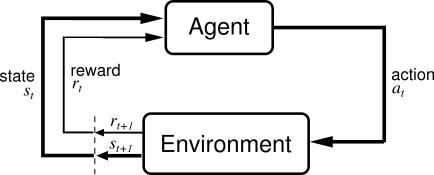
\includegraphics[width=.5\textwidth]{figures/AgentEnviornment.png}
    \caption{I am a caption}
    \label{fig:my_label}
\end{figure}


